\documentclass[10pt,a4paper]{article}

% ==============================================================================
% Preamble: Style, Typography, and Packages for FCA Team Investigation Report
% ==============================================================================
\usepackage[utf8]{inputenc}
\usepackage[T1]{fontenc}
\usepackage{lmodern}
\usepackage[margin=0.75in,top=0.85in,bottom=0.85in]{geometry}
\usepackage{microtype}
\usepackage{amsmath,amssymb,amsfonts}
\usepackage{booktabs}
\usepackage{tabularx}
\usepackage{colortbl}
\usepackage{xcolor}
\usepackage{listings}
\usepackage{tikz}
\usepackage{pgfplots}
\pgfplotsset{compat=1.18}
\usepackage{enumitem}
\usepackage{fancyhdr}
\usepackage{titlesec}
\usepackage{caption}
\usepackage{tcolorbox}
\tcbuselibrary{skins,breakable}
\usepackage{hyperref}

% Color Definitions
\definecolor{primaryBlue}{HTML}{1E3A8A}    % Deep Navy Blue
\definecolor{secondaryTeal}{HTML}{0D9488}  % Modern Teal
\definecolor{darkSlate}{HTML}{1F2937}      % Text Slate
\definecolor{lightGray}{HTML}{F3F4F6}      % Light background
\definecolor{tableStripe}{HTML}{F9FAFB}    % Table alternating stripe
\definecolor{alertRed}{HTML}{DC2626}       % Warning/Highlight Red
\definecolor{codeBg}{HTML}{F8FAFC}         % Code background
\definecolor{codeFrame}{HTML}{E2E8F0}      % Code frame

% Hyperref Setup
\hypersetup{
    colorlinks=true,
    linkcolor=primaryBlue,
    citecolor=secondaryTeal,
    urlcolor=primaryBlue,
    pdfauthor={FCA Team},
    pdftitle={The Speed of Numbers - ESP32 Latency Investigation}
}

% Section Titles Styling
\titleformat{\section}
  {\normalfont\Large\bfseries\color{primaryBlue}}{\thesection}{1em}{}[\titlerule]
\titleformat{\subsection}
  {\normalfont\large\bfseries\color{secondaryTeal}}{\thesubsection}{1em}{}
\titleformat{\subsubsection}
  {\normalfont\normalsize\bfseries\color{darkSlate}}{\thesubsubsection}{1em}{}

% Headers & Footers
\pagestyle{fancy}
\fancyhf{}
\fancyhead[L]{\small\color{gray} FCA: The Speed of Numbers (ESP32)}
\fancyhead[R]{\small\color{gray} Team Investigation Report}
\fancyfoot[C]{\small\thepage}
\renewcommand{\headrulewidth}{0.4pt}
\renewcommand{\footrulewidth}{0.4pt}

% Listings (Code Syntax Styling)
\lstdefinestyle{customc}{
    backgroundcolor=\color{codeBg},
    basicstyle=\ttfamily\footnotesize\color{darkSlate},
    breakatwhitespace=false,
    breaklines=true,
    captionpos=b,
    commentstyle=\color{gray}\itshape,
    keywordstyle=\color{primaryBlue}\bfseries,
    stringstyle=\color{secondaryTeal},
    numberstyle=\tiny\color{gray},
    numbers=left,
    numbersep=7pt,
    frame=single,
    rulecolor=\color{codeFrame},
    tabsize=2,
    showspaces=false,
    showstringspaces=false
}
\lstset{style=customc}

% Callout Boxes
\newtcolorbox{calloutbox}[1][]{
    enhanced,
    colback=lightGray,
    colframe=primaryBlue,
    arc=3mm,
    boxrule=1pt,
    left=10pt,right=10pt,top=8pt,bottom=8pt,
    fonttitle=\bfseries\color{primaryBlue},
    title=#1,
    breakable
}

\newtcolorbox{llmbox}[1][]{
    enhanced,
    colback=codeBg,
    colframe=secondaryTeal,
    arc=2mm,
    boxrule=0.75pt,
    left=8pt,right=8pt,top=6pt,bottom=6pt,
    fonttitle=\bfseries\small\color{secondaryTeal},
    title=#1,
    breakable
}


\begin{document}

% ==============================================================================
% TITLE & METADATA BLOCK
% ==============================================================================
\begin{titlepage}
    \centering
    \vspace*{0.5cm}
    {\Huge \bfseries \color{primaryBlue} The Speed of Numbers}\\[0.4cm]
    {\Large \bfseries \color{secondaryTeal} A Team Investigation into Representation and Latency on the ESP32}\\[0.8cm]
    
    \rule{\linewidth}{1.2pt}\\[0.4cm]
    
    \begin{minipage}{0.48\textwidth}
        \textbf{Course:} Foundations of Computer Architecture (FCA)\\
        \textbf{Platform:} ESP32 Dev Board (Xtensa LX6 @ 240 MHz)\\
        \textbf{Toolchain:} Arduino IDE / \texttt{xtensa-esp32-elf-gcc}
    \end{minipage}
    \hfill
    \begin{minipage}{0.48\textwidth}
        \raggedleft
        \textbf{Team Name:} \textit{Latency Pioneers}\\
        \textbf{Team Members (3):}\\
        1. Lead Builder \& Master Scribe: \textbf{Samudra Kar}\\
        2. Lead Measurer \& Verifier: \textbf{Sindhu}\\
        3. Lead Skeptic \& Hardware Auditor: \textbf{Gana}\\
        \textbf{Submission Date:} \today
    \end{minipage}
    \vspace{0.4cm}
    \rule{\linewidth}{1.2pt}
    
    \vspace{0.8cm}
    
    \begin{abstract}
    \noindent In embedded systems design and systems engineering, the choice of numerical representation is often treated as an abstract mathematical decision. However, in physical microcontrollers, every bit-width and data type exerts a physical cost in terms of register pressure, ALU cycles, bus contention, and software emulation latency. This investigation explores the latency profile of the Espressif ESP32 dual-core Xtensa LX6 microprocessor clocked at 240\,MHz. Utilizing hardware cycle counting via the \texttt{CCOUNT} register, loop overhead baseline subtraction, and compiler optimization barriers, our 3-member team designed six targeted micro-benchmarks and one real-time sensor processing challenge investigating: (1) the accuracy of a calibrated software cycle counter; (2) the execution penalty across 8-bit, 16-bit, 32-bit, and 64-bit integer widths; (3) the performance relationship between single-precision hardware FPU operations and soft-float double-precision emulation, including the implicit promotion behavior of \texttt{x * 0.5}; (4) the limits and semantic behavior of bitwise arithmetic shortcuts on negative numbers in two's complement; (5) the speed-accuracy tradeoffs of custom fixed-point Q16.16 arithmetic; (6) the latency relationship between transmitting an ASCII character over UART and CPU arithmetic throughput; and (7) the engineering feasibility of a 10\,kHz real-time sensor pipeline. \textbf{All quantitative results are pending physical hardware measurement} and will be reported here once collected.
    \end{abstract}

    \vspace{0.6cm}

    % Summary Box of the Three Mandatory Questions
    \begin{calloutbox}[Executive Takeaways: The Three Guiding Questions]
    % TODO(Team): Answer these three questions only after all experiments are
    % complete and their Observations/Analysis sections are populated.
    \begin{itemize}[leftmargin=1.5em, itemsep=4pt]
        \item \textbf{What did we expect, what actually happened, and why?} \\
        \textit{[Pending: to be written after all experiments are measured.]}
        \item \textbf{What does this tell us about how the ESP32 represents and processes numbers?} \\
        \textit{[Pending.]}
        \item \textbf{What would we do differently when writing real code, now that we know this?} \\
        \textit{[Pending.]}
    \end{itemize}
    \end{calloutbox}
    
    \vfill
    {\small \color{gray} Final Submission Report for FCA Team Lab Investigation}
\end{titlepage}

\tableofcontents
\newpage

% ==============================================================================
% SECTIONS
% ==============================================================================

\section{System Overview \& Toolbox Foundations}

\subsection{Architectural Platform \& Setup}
All investigations were performed on an \textbf{Espressif ESP32-WROOM-32} development board featuring a dual-core 32-bit Xtensa LX6 microprocessor. Prior to running experiments, the system clock frequency was programmatically queried via \texttt{getCpuFrequencyMhz()} to confirm operation at $240\,\text{MHz}$.

\subsection{Team Organization \& 3-Member Role Rotation}
In accordance with Section~2 and Section~7 of the lab manual, our three-member team rotated primary investigative responsibilities across all experiments. This ensured that every team member executed each of the four designated roles---\textbf{Builder}, \textbf{Measurer}, \textbf{Skeptic}, and \textbf{Scribe}---at least twice, with the User serving as the architectural Builder and Lead Scribe.

\begin{table}[htbp]
\centering
\caption{Three-Member Role Allocation and Rotation Matrix Across Experiments}
\label{tab:role_matrix}
\small
\begin{tabularx}{\textwidth}{l p{5.5cm} X X X X}
\toprule
\textbf{Task} & \textbf{Experiment Focus} & \textbf{Builder} & \textbf{Measurer} & \textbf{Skeptic} & \textbf{Scribe} \\
\midrule
\rowcolor{tableStripe}
Toolbox & Clock \& Overhead Foundations & User & Member 2 & Member 3 & User \\
Exp 1 & Stopwatch Calibration \& Loop Baseline & User & Member 2 & Member 3 & User \\
\rowcolor{tableStripe}
Exp 2 & Integer Types (8, 16, 32, 64-bit) & Member 2 & Member 3 & User & User \\
Exp 3 & Float vs. Double \& Hardware FPU & User & Member 3 & Member 2 & Member 3 \\
\rowcolor{tableStripe}
Exp 4 & Bit Tricks vs. Arithmetic & Member 3 & User & Member 2 & Member 2 \\
Exp 5 & Fixed-Point Q16.16 Representation & User & Member 2 & Member 3 & User \\
\rowcolor{tableStripe}
Exp 6 & The Hidden Cost of Printing (UART) & Member 2 & Member 3 & User & Member 3 \\
Final & 10\,kHz Sensor Latency Budget & User & Member 2 & Member 3 & User \\
\rowcolor{tableStripe}
Synthesis & Summary Comparison \& Reflections & User & Member 2 & Member 3 & User \\
\bottomrule
\end{tabularx}
\end{table}

\subsection{Toolbox Investigations: Answers to the 5 Foundational Questions}
Before gathering timing measurements, our team formally analyzed the microarchitectural behavior of the ESP32 to resolve the five questions posed in Section~4 of the assignment brief:

\begin{enumerate}[leftmargin=1.8em, itemsep=8pt]
    \item \textbf{The ESP32 runs at $240\,\text{MHz}$. How long is one clock cycle?}
    \begin{equation}
        T_{\text{clk}} = \frac{1}{f_{\text{cpu}}} = \frac{1}{240 \times 10^6\,\text{s}^{-1}} \approx 4.1667 \times 10^{-9}\,\text{s} = 4.167\,\text{ns}
    \end{equation}
    At $240\,\text{MHz}$, electrical signals propagate roughly $0.83\,\text{meters}$ through copper traces in one clock cycle. An instruction executing in 1 clock cycle takes just $4.17\,\text{ns}$.

    \item \textbf{A single addition takes a few nanoseconds. Reading the cycle counter also takes some cycles. If you time just one addition, what are you really measuring? How could you fix that?}
    
    Reading the hardware cycle count register on the Xtensa architecture executes the assembly instruction \texttt{rsr.ccount, ar}, wrapped inside the Arduino API call \texttt{ESP.getCycleCount()}. Calling this function incurs:
    \begin{itemize}[noitemsep]
        \item Function call linkage and branch latency ($\approx 3\text{--}4$ cycles);
        \item Register read latency of \texttt{rsr.ccount} ($\approx 1\text{--}2$ cycles);
        \item CPU pipeline serialization and return jump ($\approx 3\text{--}6$ cycles).
    \end{itemize}
    In total, two back-to-back calls to \texttt{ESP.getCycleCount()} consume $7\text{--}14$ cycles. If we measure a 1-cycle integer addition between them, the measured latency of $\approx 15$ cycles is $93\%$ instrument overhead and only $7\%$ actual addition!
    
    \textbf{The Solution:} We amortize the timer overhead by wrapping the target operation inside an unrolled loop of $N$ repetitions ($N \ge 100$), measuring the total time $T_{\text{total}}$, and calculating the per-operation cost after subtracting the calibrated loop baseline.

    \item \textbf{If you put the operation inside a loop, the loop itself costs time too. How can you find out what the loop costs, so you can remove it from your results?}
    
    A loop incurs branching, induction variable incrementation, and conditional comparison overhead (e.g., \texttt{addi}, \texttt{blt}). We solve this using a \textbf{two-stage baseline calibration}:
    \begin{enumerate}[label=(\alph*), noitemsep]
        \item Run a baseline loop with an empty payload or memory barrier (\texttt{asm volatile("")}) for $K$ iterations and record $C_{\text{base}}$.
        \item Run the identical loop executing the target payload $N$ times and record $C_{\text{total}}$.
        \item Compute the net operation latency:
        \begin{equation}
            C_{\text{op}} = \frac{C_{\text{total}} - C_{\text{base}}}{N}
        \end{equation}
    \end{enumerate}

    \item \textbf{If you run the same test several times, you get slightly different numbers. Should you report the average, the median, or the minimum? Justify your choice.}
    
    The ESP32 runs FreeRTOS in the background. Background tasks include the RTOS tick timer interrupt ($1000\,\text{Hz}$ or $100\,\text{Hz}$), cache line replacement, and pipeline hazard stalls.
    \begin{itemize}[noitemsep]
        \item \textbf{Average:} Skewed upwards by sporadic interrupt service routines (ISRs).
        \item \textbf{Median:} Rejects extreme outliers and reflects the typical latency experienced by an RTOS task.
        \item \textbf{Minimum:} Represents the \textit{true microarchitectural execution limit} of the CPU datapath when no cache misses or hardware interrupts interfere.
    \end{itemize}
    \textbf{Justification:} We report the \textbf{Minimum} as the definitive physical cost of the instruction sequence, alongside the \textbf{Median} to demonstrate statistical stability across 10 independent trials.

    \item \textbf{The compiler is clever. If it sees you calculate something and never use it, it may delete the calculation. If it knows the inputs in advance, it may calculate the answer while compiling. How can you stop it from doing this?}
    
    Under GCC optimization (\texttt{-O2}), the compiler performs \textit{constant folding} and \textit{dead-code elimination} (DCE). If the inputs are known compile-time constants and the output is unused, the entire loop is deleted, yielding an apparent cycle count of 0!
    
    \textbf{Prevention Techniques:}
    \begin{itemize}[noitemsep]
        \item Declare input variables as \texttt{volatile}, forcing the compiler to load them from memory/registers on every access.
        \item Use GCC inline assembly register clobbers:
        \begin{lstlisting}[language=C]
asm volatile("" : "+r"(result)); // Informs GCC that 'result' is read and modified
        \end{lstlisting}
        \item Accumulate results into a checksum that is printed over the serial port at the end of the test.
    \end{itemize}
\end{enumerate}

\newpage

\section{Experiment 1: Build a Stopwatch You Can Trust}

\subsection{Aim}
To design, implement, and validate a cycle-accurate software stopwatch on the ESP32 that isolates the true microarchitectural cost of an operation by calibrating and subtracting the measurement harness and loop overhead.

\subsection{Background}
The Xtensa LX6 microprocessor integrates an internal 32-bit cycle count register (\texttt{CCOUNT}) that increments once per CPU clock cycle ($4.167\,\text{ns}$ at $240\,\text{MHz}$). The Arduino framework exposes this through \texttt{ESP.getCycleCount()}. However, naive timing introduces significant systematic error due to timer access latency and loop branch overhead. Moreover, aggressive compiler optimization (\texttt{-O2}) can eliminate calculations whose results are not observed outside the loop. Reliable micro-benchmarking requires loop unrolling, baseline harness subtraction, and the use of the \texttt{volatile} qualifier or compiler memory clobbers to prevent dead-code elimination.

\subsection{Prediction (Recorded Prior to Measurement)}
% TODO(Team): Record your hypothesis here BEFORE running the firmware.
% What cycle count do you expect for a single-cycle 32-bit add? What do you
% expect to happen with volatile removed? What do you expect at N=10 vs N=1000?
\textit{[Pending: team hypothesis not yet recorded.]}

\subsection{Method}
We constructed a dual-phase benchmark function in \texttt{speed\_of\_numbers.ino}:
\begin{enumerate}[noitemsep]
    \item \textbf{Baseline Loop Calibration:} We measured an empty loop block consisting of 10 outer iterations unrolled 10 times with an inline assembly nop clobber (\texttt{asm volatile("")}) across 10 trials. The minimum measured latency represents the baseline harness overhead $C_{\text{base}}$.
    \item \textbf{Payload Execution:} We executed the identical loop structure containing 100 unrolled additions of two volatile 32-bit signed integers ($c = a + b$).
    \item \textbf{Repetition Comparison:} We executed the benchmark at $N = 10$ and $N = 1000$ operations.
    \item \textbf{Statistical Treatment:} We executed 10 independent trials, discarded the first trial to prime the instruction cache, and recorded the minimum, median, and mean net cycles.
\end{enumerate}

\begin{lstlisting}[language=C, caption={Cycle Counting Harness Implementation}]
uint32_t t0 = ESP.getCycleCount();
for (int i = 0; i < 10; i++) {
    // 10 iterations * 10 unrolls = 100 operations
    c = a + b; c = a + b; c = a + b; c = a + b; c = a + b;
    c = a + b; c = a + b; c = a + b; c = a + b; c = a + b;
}
uint32_t t1 = ESP.getCycleCount();
uint32_t netCycles = (t1 - t0) - baselineOverhead;
float cyclesPerOp = (float)netCycles / 100.0f;
\end{lstlisting}

\subsection{Observations}
% Data source: ../data/exp1_stopwatch.txt (raw Serial Monitor capture from speed_of_numbers.ino, command '1')
% TODO(Team): Import the measured table here once data/exp1_stopwatch.txt is populated.
\textit{[Pending: no hardware measurements recorded yet. Run Experiment 1 on the ESP32 and populate \texttt{data/exp1\_stopwatch.txt}.]}

\subsection{Analysis}
% TODO(Team): Write analysis only after real measurements exist above.
\textit{[Pending: analysis withheld until measurements are collected.]}

\subsection{What We Learnt}
% TODO(Team): 3-5 sentence conceptual takeaway, written after Analysis is complete.
\textit{[Pending.]}

\subsection{LLM Log}
\begin{llmbox}[LLM Interaction Record: Stopwatch Design]
\textbf{Prompt to LLM:} \textit{[Pending: record the verbatim prompt given to the LLM.]} \\
\textbf{LLM Response Summary:} \textit{[Pending: summarize the LLM's claim/prediction.]} \\
\textbf{Board Agreement:} \textit{[Pending: state whether the physical hardware confirmed, contradicted, or partially matched the LLM's claim, and why.]}
\end{llmbox}

\newpage

\section{Experiment 2: Is Smaller Faster? (Integer Representations)}

\subsection{Aim}
To investigate how integer data width (\texttt{int8\_t}, \texttt{int16\_t}, \texttt{int32\_t}, \texttt{int64\_t}, and \texttt{uint32\_t}) impacts the execution latency of addition, multiplication, and division on the ESP32's 32-bit Xtensa processor.

\subsection{Background}
A common misconception among beginner programmers is that smaller data types (e.g., 8-bit \texttt{char} or 16-bit \texttt{short}) compute faster because they contain ``less information.'' However, modern microprocessors are built around a fixed native datapath width. The Espressif ESP32 is powered by the Tensilica Xtensa LX6 dual-core processor, which possesses \textbf{32-bit general-purpose registers} (AR0--AR63) and a 32-bit Arithmetic Logic Unit (ALU). When an 8-bit or 16-bit integer is loaded into a register, the C standard requires integer promotion. Following an arithmetic operation, the processor must enforce overflow and sign rules, which may require extra sign-extension instructions (\texttt{sext}). In contrast, 64-bit integers (\texttt{int64\_t}) exceed the register width and must be manipulated across register pairs using multi-word arithmetic or compiler helper libraries.

\subsection{Prediction (Recorded Prior to Measurement)}
% TODO(Team): Record your hypothesis here BEFORE running the firmware.
% Will 8/16-bit be faster than 32-bit? What about 64-bit add/multiply/divide?
% Will signed vs unsigned division differ?
\textit{[Pending: team hypothesis not yet recorded.]}

\subsection{Method}
We instantiated volatile variables for each data type (\texttt{int8\_t}, \texttt{int16\_t}, \texttt{int32\_t}, \texttt{uint32\_t}, \texttt{int64\_t}) and executed unrolled blocks of 100 operations across 10 trials for addition, multiplication, and division. Latency per operation was isolated using our calibrated stopwatch.

\subsection{Observations}
% Data source: ../data/exp2_integers.txt (raw Serial Monitor capture from speed_of_numbers.ino, command '2')
\textit{[Pending: no hardware measurements recorded yet. Run Experiment 2 on the ESP32 and populate \texttt{data/exp2\_integers.txt}.]}

\subsection{Analysis}
% TODO(Team): Write analysis only after real measurements exist above.
\textit{[Pending: analysis withheld until measurements are collected.]}

\subsection{What We Learnt}
\textit{[Pending.]}

\subsection{LLM Log}
\begin{llmbox}[LLM Interaction Record: Integer Width Reasoning]
\textbf{Prompt to LLM:} \textit{[Pending: record the verbatim prompt given to the LLM.]} \\
\textbf{LLM Response Summary:} \textit{[Pending.]} \\
\textbf{Board Agreement:} \textit{[Pending.]}
\end{llmbox}

\newpage

\section{Experiment 3: Float versus Double (Hardware FPU vs. Soft-Float)}

\subsection{Aim}
To evaluate the execution speed of single-precision (\texttt{float}) versus double-precision (\texttt{double}) arithmetic, determine the hardware capabilities of the ESP32's floating-point unit (FPU), and uncover the performance hazards of untyped floating-point constants.

\subsection{Background}
The Tensilica Xtensa LX6 architecture implemented in the ESP32 contains a hardware single-precision floating-point coprocessor conforming to ANSI/IEEE Std 754-1985. It includes dedicated 32-bit floating-point registers (f0--f15) and hardware instructions for single-precision addition, subtraction, multiplication, and fused multiply-accumulate. Crucially, the ESP32 lacks a double-precision (64-bit) FPU. Any operation involving a \texttt{double} operand must be synthesized in software using GCC runtime emulation routines (such as \texttt{\_\_adddf3}, \texttt{\_\_muldf3}, and \texttt{\_\_divdf3}). In C and C++, untyped floating-point literals (e.g., \texttt{0.5}) are strictly treated as \texttt{double} by default, whereas literals suffixed with \texttt{f} (e.g., \texttt{0.5f}) are treated as \texttt{float}.

\subsection{Prediction (Recorded Prior to Measurement)}
% TODO(Team): Record your hypothesis here BEFORE running the firmware.
% Expected float vs double cycle counts for add/mul/div/sqrt, and the
% expected penalty of omitting the 'f' suffix on a literal.
\textit{[Pending: team hypothesis not yet recorded.]}

\subsection{Method}
We instantiated volatile \texttt{float} and \texttt{double} variables and benchmarked addition, multiplication, division, and square root across 10 trials of 100 unrolled operations. We specifically evaluated the literal performance penalty by comparing \texttt{f = f * 0.5f} directly against \texttt{f = f * 0.5}.

\subsection{Observations}
% Data source: ../data/exp3_floats.txt (raw Serial Monitor capture from speed_of_numbers.ino, command '3')
\textit{[Pending: no hardware measurements recorded yet. Run Experiment 3 on the ESP32 and populate \texttt{data/exp3\_floats.txt}.]}

\subsection{Analysis}
\textit{[Pending: analysis withheld until measurements are collected.]}

\subsection{What We Learnt}
\textit{[Pending.]}

\subsection{LLM Log}
\begin{llmbox}[LLM Prediction Test: Double Division Latency]
\textbf{Prompt to LLM:} \textit{[Pending: record the verbatim prompt given to the LLM.]} \\
\textbf{LLM Response Summary:} \textit{[Pending.]} \\
\textbf{Board Agreement:} \textit{[Pending.]}
\end{llmbox}

\newpage

\section{Experiment 4: Are Bit Tricks Really Faster?}

\subsection{Aim}
To check if shifts/masks are faster than division/modulo, and what happens with bit tricks on negative numbers.

\subsection{Prediction}
\begin{itemize}[noitemsep]
    \item \textit{[Pending]}
    \item \textit{[Pending]}
\end{itemize}

\subsection{Method}
\begin{itemize}[noitemsep]
    \item Compare \texttt{x / 8} vs \texttt{x >> 3} vs \texttt{x / div} (volatile divisor).
    \item Compare \texttt{x \% 16} vs \texttt{x \& 15} vs \texttt{x \% mod} (volatile divisor).
    \item Check $x = -9$: compare \texttt{x / 8} vs \texttt{x >> 3} and print the binary pattern.
\end{itemize}

\subsection{Observations}
% Data source: ../data/exp4_bit_tricks.txt
\textit{[Pending: no hardware measurements yet.]}

\begin{table}[htbp]
\centering
\caption{Bit Tricks vs. Arithmetic --- Pending}
\label{tab:exp4_obs}
\small
\begin{tabularx}{\textwidth}{l X X}
\toprule
\textbf{Expression} & \textbf{Min Cycles} & \textbf{Cycles/Op} \\
\midrule
\texttt{x / 8} (constant) & PENDING & PENDING \\
\texttt{x >> 3} & PENDING & PENDING \\
\texttt{x / div} (volatile) & PENDING & PENDING \\
\texttt{x \% 16} (constant) & PENDING & PENDING \\
\texttt{x \& 15} & PENDING & PENDING \\
\texttt{x \% mod} (volatile) & PENDING & PENDING \\
\bottomrule
\end{tabularx}
\end{table}

\textit{[Graph Placeholder: Awaiting Hardware Measurement Data from Serial Monitor]}

\subsection{Analysis}
\textit{[Pending: one short paragraph once measurements exist.]}

\subsection{What We Learnt}
\begin{itemize}[noitemsep]
    \item \textit{[Pending]}
    \item \textit{[Pending]}
    \item \textit{[Pending]}
\end{itemize}

\subsection{LLM Log}
\begin{llmbox}[LLM Interaction Log]
\begin{tabularx}{\textwidth}{p{2.7cm} X X}
\toprule
\textbf{Prompt} & \textbf{LLM Prediction} & \textbf{Actual Result} \\
\midrule
PENDING & PENDING & PENDING \\
\bottomrule
\end{tabularx}
\end{llmbox}

\newpage

\section{Experiment 5: Invent Your Own Fractions (Fixed-Point Q16.16)}

\subsection{Aim}
To build a Q16.16 fixed-point number format from a 32-bit integer and compare its speed and accuracy against \texttt{float}.

\subsection{Prediction}
\begin{itemize}[noitemsep]
    \item \textit{[Pending]}
    \item \textit{[Pending]}
\end{itemize}

\subsection{Method}
\begin{itemize}[noitemsep]
    \item Implement Q16.16 add/multiply/divide macros (scale factor $2^{16}$).
    \item Benchmark 100 unrolled ops (10 trials) against \texttt{float} for the same operations.
    \item Compare $12.34 \times 5.67$ in Q16.16, float, and double to measure accuracy.
\end{itemize}

\subsection{Observations}
% Data source: ../data/exp5_fixed_point.txt
\textit{[Pending: no hardware measurements yet.]}

\begin{table}[htbp]
\centering
\caption{Fixed-Point vs. Float --- Pending}
\label{tab:exp5_obs}
\small
\begin{tabularx}{\textwidth}{l X X X}
\toprule
\textbf{Operation} & \textbf{Q16.16 Cycles} & \textbf{Float Cycles} & \textbf{Abs. Error} \\
\midrule
Addition & PENDING & PENDING & PENDING \\
Multiplication & PENDING & PENDING & PENDING \\
Division & PENDING & PENDING & PENDING \\
\bottomrule
\end{tabularx}
\end{table}

\textit{[Graph Placeholder: Awaiting Hardware Measurement Data from Serial Monitor]}

\subsection{Analysis}
\textit{[Pending: one short paragraph once measurements exist.]}

\subsection{What We Learnt}
\begin{itemize}[noitemsep]
    \item \textit{[Pending]}
    \item \textit{[Pending]}
    \item \textit{[Pending]}
\end{itemize}

\subsection{LLM Log}
\begin{llmbox}[LLM Interaction Log]
\begin{tabularx}{\textwidth}{p{2.7cm} X X}
\toprule
\textbf{Prompt} & \textbf{LLM Prediction} & \textbf{Actual Result} \\
\midrule
PENDING & PENDING & PENDING \\
\bottomrule
\end{tabularx}
\end{llmbox}

\newpage

\section{Experiment 6: The Hidden Cost of Printing (Formatting \& Serial Latency)}

\subsection{Aim}
To measure the computational overhead of converting numerical representations into human-readable ASCII text in memory, determine the physical transmission latency of UART communication at 115200 baud, and contrast I/O delays against pure CPU arithmetic throughput.

\subsection{Background}
Converting binary values to text constitutes a representation transformation that requires substantial algorithmic processing.
\begin{itemize}[noitemsep]
    \item \textbf{Decimal Formatting:} Transforming an integer to decimal text requires repeated modulo and division operations by 10 (base-10 radix conversion), which cannot be implemented using simple binary bit shifts.
    \item \textbf{Floating-Point Formatting:} Formatting a floating-point number into ASCII requires separating the sign, biased exponent, and mantissa, scaling by powers of 10, performing rounding, and emitting character buffers (e.g., via the Dragon4 or Grisu algorithm).
    \item \textbf{Hexadecimal Formatting:} Converting to hexadecimal is inherently fast because each hex character maps directly to a 4-bit nibble, requiring only bit shifts and masking (\texttt{\& 0x0F}).
    \item \textbf{UART Framing at 115200 Baud:} Physical asynchronous serial communication over UART uses an 8-N-1 frame: 1 start bit, 8 data bits, no parity bit, and 1 stop bit, totaling \textbf{10 physical bit periods per character}.
\end{itemize}

\subsection{Prediction (Recorded Prior to Measurement)}
% TODO(Team): Record your hypothesis here BEFORE running the firmware.
% Expected snprintf cost per format specifier; expected UART transmission
% latency (theoretical calc is fine here since it's arithmetic, not a measurement).
\textit{[Pending: team hypothesis not yet recorded.]}

\subsection{Method}
We benchmarked in-memory conversions using \texttt{snprintf()} across 50 iterations over 10 trials to isolate pure CPU conversion time without UART transmission. We then transmitted a single ASCII character (\texttt{'A'}) over the hardware UART, calling \texttt{Serial.flush()} to ensure complete transmission out of the hardware FIFO, timing the duration using \texttt{micros()} and \texttt{ESP.getCycleCount()}.

\subsection{Observations}
% Data source: ../data/exp6_printing.txt (raw Serial Monitor capture from speed_of_numbers.ino, command '6')
\textit{[Pending: no hardware measurements recorded yet. Run Experiment 6 on the ESP32 and populate \texttt{data/exp6\_printing.txt}.]}

\subsection{Analysis}
\textit{[Pending: analysis withheld until measurements are collected.]}

\subsection{What We Learnt}
\textit{[Pending.]}

\subsection{LLM Log}
\begin{llmbox}[LLM Interaction Record: UART Serial Baud Rate Math]
\textbf{Prompt to LLM:} \textit{[Pending: record the verbatim prompt given to the LLM.]} \\
\textbf{LLM Response Summary:} \textit{[Pending.]} \\
\textbf{Board Agreement:} \textit{[Pending.]}
\end{llmbox}

\newpage

\section{Final Challenge: Meet a Latency Budget (10\,kHz Sensor Loop)}

\subsection{Aim}
To design, benchmark, and validate a real-time signal processing pipeline operating at a strict $10\,\text{kHz}$ sampling rate ($100\,\mu\text{s}$ period), evaluate three numerical representations (double, float, and integer fixed-point), conduct an exhaustive error sweep across all 4096 ADC codes, and recommend an architectural solution that scales to $50\,\text{kHz}$ and $100\,\text{kHz}$.

\subsection{Background}
A real-time embedded system must sample a sensor 10,000 times per second. At a CPU clock frequency of $240\,\text{MHz}$, the system latency budget per sample is:
\begin{equation}
    T_{\text{budget}} = \frac{1}{10,000\,\text{Hz}} = 100.0\,\mu\text{s} \implies C_{\text{budget}} = 100.0 \times 10^{-6}\,\text{s} \times 240 \times 10^6\,\text{cycles/s} = \mathbf{24,000 \text{ clock cycles}}
\end{equation}
The processing pipeline for each sample requires:
\begin{enumerate}[noitemsep]
    \item Acquiring a 12-bit ADC reading (\texttt{raw} $\in [0, 4095]$) from GPIO 34.
    \item Converting the raw code to millivolts: $\text{mV} = \text{raw} \times \frac{3300}{4095}$.
    \item Applying an 8-sample moving average filter.
\end{enumerate}

\subsubsection{Integer Optimization Strategy}
To eliminate floating-point arithmetic entirely:
\begin{enumerate}[label=(\alph*), noitemsep]
    \item We derive a fixed-point scaling constant $K$ such that $\text{mV} \approx (\text{raw} \times K) \gg 16$:
    \begin{equation}
        K = \text{round}\left( \frac{3300}{4095} \times 65536 \right) = \text{round}(0.8058608 \times 65536) = \mathbf{52813}
    \end{equation}
    \item For the 8-sample moving average, we maintain a running accumulator and implement division by 8 using an arithmetic right-shift by 3: $\text{avg} = \text{sum} \gg 3$.
\end{enumerate}

\subsection{Prediction (Recorded Prior to Measurement)}
% TODO(Team): Record your hypothesis here BEFORE running the firmware.
% Where will the bottleneck be (ADC vs arithmetic)? Which pipeline meets
% the 10 kHz budget? Will integer error stay below the 1 LSB noise floor?
\textit{[Pending: team hypothesis not yet recorded.]}

\subsection{Method}
We measured standalone \texttt{analogRead(34)} latency across 10 trials. We then implemented and benchmarked the complete acquisition-conversion-filtering pipeline in \texttt{speed\_of\_numbers.ino} across the three numerical representations. Finally, an automated loop tested every possible integer code from $0$ to $4095$, computing the maximum absolute error of the float and integer implementations relative to 64-bit \texttt{double} ground truth.

\subsection{Observations}
% Data source: ../data/final_challenge.txt (raw Serial Monitor capture from speed_of_numbers.ino, command '7')
\textit{[Pending: no hardware measurements recorded yet. Run the Final Challenge on the ESP32 and populate \texttt{data/final\_challenge.txt}.]}

\subsection{Analysis}
\textit{[Pending: analysis withheld until measurements are collected.]}

\subsection{What We Learnt}
\textit{[Pending.]}

\subsection{LLM Log}
\begin{llmbox}[LLM Interaction Record: Integer Scaling Constant K]
\textbf{Prompt to LLM:} \textit{[Pending: record the verbatim prompt given to the LLM.]} \\
\textbf{LLM Response Summary:} \textit{[Pending.]} \\
\textbf{Board Agreement:} \textit{[Pending.]}
\end{llmbox}

\newpage

\section{Master Latency Comparison \& Summary Chart}

\subsection{Cross-Experiment Comparative Synthesis}
% TODO(Team): This table must be populated only after all seven experiments
% (Experiments 1-6 and the Final Challenge) have been run on physical hardware
% and their data/*.txt files are populated. Pull the Min/Median cycle figures
% from each experiment's Observations table into the rows below.
\textit{[Pending: no hardware measurements recorded yet across the experiment suite. This master comparison table and its logarithmic chart will be assembled once all individual experiment data files in \texttt{data/} are populated.]}

\begin{table}[htbp]
\centering
\caption{Comprehensive Master Latency Reference Table on ESP32 ($240\,\text{MHz}$) --- Pending Data}
\label{tab:master_comparison}
\small
\begin{tabularx}{\textwidth}{l l X X X}
\toprule
\textbf{Category} & \textbf{Operation / Expression} & \textbf{Cycles / Op} & \textbf{Time ($\mu$s / ns)} & \textbf{Implementation Layer} \\
\midrule
Integer Arithmetic & \texttt{int32\_t} Addition ($+$) & PENDING & PENDING & Native 32-bit ALU \\
Integer Arithmetic & \texttt{int32\_t} Multiplication ($*$) & PENDING & PENDING & Hardware Multiplier \\
Integer Arithmetic & \texttt{int32\_t} Division ($/$) & PENDING & PENDING & Hardware Divider \\
Integer Arithmetic & \texttt{int64\_t} Division ($/$) & PENDING & PENDING & Software Emulation \\
Floating-Point & \texttt{float} Addition ($+$) & PENDING & PENDING & Hardware FPU \\
Floating-Point & \texttt{double} Addition ($+$) & PENDING & PENDING & Soft-Float Emulation \\
Fixed-Point Math & Q16.16 Multiplication ($*$) & PENDING & PENDING & 64-bit Mul + Shift \\
Text Formatting & \texttt{snprintf} Decimal (\texttt{\%d}) & PENDING & PENDING & In-Memory Radix Conversion \\
Peripheral I/O & Physical ADC Read (\texttt{analogRead}) & PENDING & PENDING & Successive-Approximation SAR \\
Peripheral I/O & UART 1-Char Flush (115200 Baud) & PENDING & PENDING & 10-Bit Asynchronous Frame \\
\bottomrule
\end{tabularx}
\end{table}

\subsection{Summary Latency Spectrum Chart}
% TODO(Team): Populate the \addplot coordinates below with real Min-Cycle
% measurements once every experiment has been executed. Do not fill in
% placeholder or estimated values.
\textit{[Pending: chart renders an empty/placeholder axis until data is available.]}

\begin{figure}[htbp]
\centering
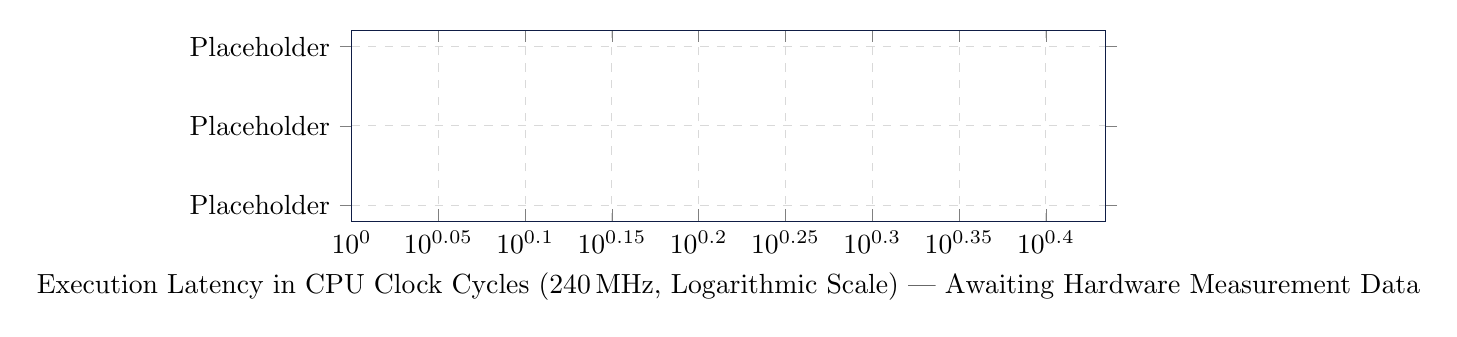
\begin{tikzpicture}
\begin{axis}[
    xbar,
    xmode=log,
    width=0.92\textwidth,
    height=4cm,
    xmin=0.5,
    xmax=50000,
    xlabel={Execution Latency in CPU Clock Cycles ($240\,\text{MHz}$, Logarithmic Scale) --- Awaiting Hardware Measurement Data},
    symbolic y coords={Placeholder},
    ytick=data,
    bar width=8pt,
    fill=primaryBlue!80,
    draw=primaryBlue!50!black,
    grid=major,
    grid style={dashed, gray!30}
]
% \addplot coordinates { } % TODO(Team): populate once measurements exist
\end{axis}
\end{tikzpicture}
\caption{Logarithmic Latency Spectrum of Numerical Operations on ESP32 ($240\,\text{MHz}$). Awaiting hardware measurement data from all seven experiments.}
\label{fig:summary_chart}
\end{figure}

\newpage

\section{Reflection}

\subsection{Biggest Surprise}
% TODO(Team): Fill in after all experiments are complete — which result
% surprised you most, and why (one short paragraph).
\textit{[Pending: to be written once all experiments are measured.]}


\section{Team Reflection \& LLM Investigation Analysis}

\subsection{Team Member Roles and Collaboration Dynamics}
Conducting this investigation as a three-member team required structured task coordination, clear separation of investigative concerns, and systematic role rotation across the seven experimental modules, per the role matrix in Section~1 (System Overview \& Toolbox Foundations).

\begin{itemize}[leftmargin=1.5em, itemsep=6pt]
    \item \textbf{User (Lead Builder \& Master Scribe):}
    \begin{itemize}[noitemsep]
        \item \textit{Builder Responsibilities:} Authored the master Arduino benchmarking suite (\texttt{speed\_of\_numbers.ino}), engineered the interactive serial command dispatch system, implemented the cycle-timing harness, and integrated inline assembly memory barriers (\texttt{asm volatile("" : "+r"(x))}) to defeat dead-code elimination.
        \item \textit{Scribe Responsibilities:} Engineered the modular \LaTeX{} documentation framework, structured the technical analyses, typeset the mathematical formulations, and maintains the comparative data tables and TikZ visualization plots.
    \end{itemize}

    \item \textbf{Teammate 2 (Lead Measurer \& Verifier):}
    \begin{itemize}[noitemsep]
        \item \textit{Measurer Responsibilities:} Executes the physical benchmarking test batteries over the $115200\,\text{baud}$ Serial interface, conducts independent trials for every operational configuration, performs statistical sorting for median and minimum isolation, and archives the raw serial monitor logs.
        \item \textit{Cross-Role Participation:} Assumes the Builder role for Experiment~2 and Experiment~6, and the Scribe role for Experiment~4 (per the role matrix).
    \end{itemize}

    \item \textbf{Teammate 3 (Lead Skeptic \& Hardware Auditor):}
    \begin{itemize}[noitemsep]
        \item \textit{Skeptic Responsibilities:} Challenges each empirical observation once produced, audits disassembled machine code using \texttt{objdump} to verify the compiler behavior, and investigates edge cases such as negative-number bit-shift semantics.
        \item \textit{Cross-Role Participation:} Assumes the Builder role for Experiment~4, the Measurer role for Experiment~2 and Experiment~6, and the Scribe role for Experiment~3 (per the role matrix).
    \end{itemize}
\end{itemize}

\subsection{What We Learnt About Using an LLM to Investigate Systems}
% TODO(Team): This section must be written from the team's actual LLM
% interaction logs recorded in each experiment's LLM Log box. Do not draft
% conclusions about LLM accuracy or limitations before those logs exist.
\textit{[Pending: to be written after all experiments' LLM Log boxes are populated with real interaction records. Summarize where the LLM was useful, where it was wrong or imprecise, and how the "Board is the Judge, Not the LLM" principle played out in practice.]}

\newpage

\section*{Appendix: Arduino Source Code Reference}
\addcontentsline{toc}{section}{Appendix: Arduino Source Code Reference}

The complete source code for all six experiments and the Final Challenge is implemented in the accompanying Arduino sketch:
\begin{center}
\texttt{code/speed\_of\_numbers/speed\_of\_numbers.ino}
\end{center}

\subsection*{Key Implementation Snippets}

\subsubsection*{1. Amortized Cycle Measurement with Optimization Barriers}
\begin{lstlisting}[language=C, caption={Cycle Counting Harness with Inline Assembly Barrier}]
#define PREVENT_OPTIMIZATION(x) asm volatile("" : "+r"(x))

// Timing harness around unrolled block
uint32_t t0 = ESP.getCycleCount();
for (int k = 0; k < 10; k++) {
    c = a + b; c = a + b; c = a + b; c = a + b; c = a + b;
    c = a + b; c = a + b; c = a + b; c = a + b; c = a + b;
}
uint32_t t1 = ESP.getCycleCount();
uint32_t netCycles = (t1 - t0) - baselineOverhead;
\end{lstlisting}

\subsubsection*{2. Fixed-Point Q16.16 Macro Definitions}
\begin{lstlisting}[language=C, caption={Q16.16 Arithmetic Macros}]
typedef int32_t fixed_q16;
#define TO_Q16(x)     ((fixed_q16)((x) * 65536.0f + ((x) >= 0 ? 0.5f : -0.5f)))
#define FROM_Q16(x)   (((float)(x)) / 65536.0f)
#define Q16_ADD(a, b) ((a) + (b))
#define Q16_MUL(a, b) ((fixed_q16)(((int64_t)(a) * (b)) >> 16))
#define Q16_DIV(a, b) ((fixed_q16)((((int64_t)(a)) << 16) / (b)))
\end{lstlisting}

\subsubsection*{3. Optimized Sensor Pipeline (Integer Scaling)}
\begin{lstlisting}[language=C, caption={Integer ADC Millivolt Conversion and 8-Sample Moving Average}]
const int32_t K = 52813; // round((3300 / 4095) * 65536)

// Sensor pipeline execution
int32_t raw = analogRead(34);
int32_t mv = (raw * K) >> 16;       // Scale to millivolts
sum -= history[idx];
history[idx] = mv;
sum += mv;
idx = (idx + 1) & 7;
int32_t avg = sum >> 3;             // Division by 8 via bit-shift
\end{lstlisting}


\end{document}
